\subsection{Cache Memory}

Cache memory is transparent (hidden) to the software and is managed by the hardware.
It stores copies of frequently accessed data to speed up subsequent access to that data.

There can be one or more layers between the CPU and main memory.
The transfer between the CPU and L1 cache is the fastest, and the speed decreases
as the distance from the CPU increases.

\subsubsection{Cache Memory Organisation}

A word-addressable main memory with $n$-bit addresses has $2^n$ words. Divide the
main memory into blocks of $K$ words each, then the memory has $M=\frac{2^n}{K}$ blocks.
Suppose the cache has $m$ blocks, called \textbf{lines}. Generally, we have $m \ll M$.
Each line has $K$ words, a tag, and several control bits. The length of the line,
excluding the tag and the control bits is called the \textbf{line size} or
\textbf{block length}.

\begin{figure}[H]
\centering
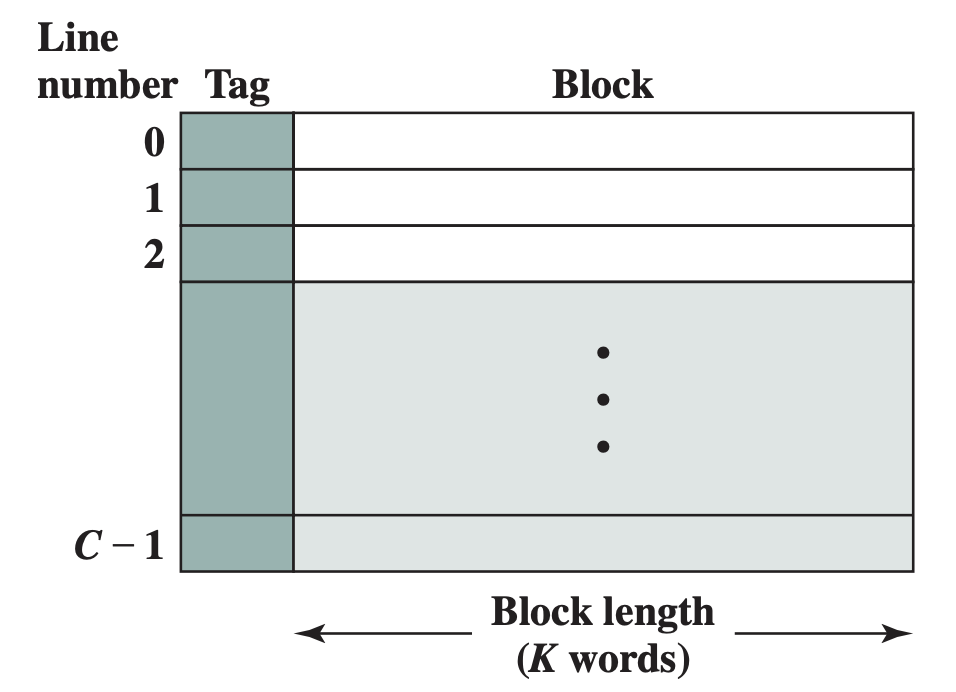
\includegraphics[width=0.4\linewidth]{chaps/memory/cache-memory/cache-mem-organisation.png}
\caption{Cache Memory Organisation}
\end{figure}

\subsubsection{Cache Memory Read}

The process of reading from the cache is roughly described as follows:
\begin{enumerate}
    \item Obtain the address of the word to be read from the CPU.
    \item Check if the block containing the word is in the cache.
    \begin{enumerate}
        \item If the block is in the cache, read the word from the cache.
        \item If the block is not in the cache, load the block from the main memory
            into the cache, and \textbf{at the same time} deliver the word to the CPU.
    \end{enumerate}
\end{enumerate}

\subsubsection{Address Mapping}

There are three ways to map the main memory to the cache:
\begin{enumerate}
\item \textbf{Direct Mapping}: 
    Each block of main memory maps to exactly one line in the cache. The mapping is
    given as $i = j\mod m$, where $i$ is the cache line number, $j$ is the main memory
    block number, and $m$ is the number of cache lines.
    
    \begin{example}
        The cache logic treats the main memory address in three parts as follows:
        \begin{equation*}
            \underbrace{0000\,0001}_{(s-r)\text{ bits (tag)}}\,
            \overbrace{1111\,1111\,1111\,11}^{r\text{ bits (line number)}}
            \underbrace{00}_{w\text{ bits (word)}}
        \end{equation*}
        The least significant $w$ bits identify the word within the block,
        where the block size is $2^w$ words. The next $r$ bits identify the line
        number within the cache memory, where the cache memory has $2^r$ lines.
        The most significant $(s-r)$ bits are the tag bits, which are used to
        distinguish between the different main memory blocks that map to the same line,
        where the main memory has $2^s$ blocks.
    \end{example}

    To perform a read operation, the line number first identifies the line in the cache.
    Then, the tag bits in the line are compared with the tag bits in the address.
    If the tags match, the word is read from the cache according to the word bits in the
    address. If the tags do not match, the block is read from the main memory into the
    cache, and the word is read from the cache.

\item \textbf{Fully Associative Mapping}:


\item \textbf{Set Associative Mapping}:


\end{enumerate}